% Options for packages loaded elsewhere
\PassOptionsToPackage{unicode}{hyperref}
\PassOptionsToPackage{hyphens}{url}
%
\documentclass[
  a4paper,
]{article}
\usepackage{amsmath,amssymb}
\usepackage{setspace}
\usepackage{iftex}
\ifPDFTeX
  \usepackage[T1]{fontenc}
  \usepackage[utf8]{inputenc}
  \usepackage{textcomp} % provide euro and other symbols
\else % if luatex or xetex
  \usepackage{unicode-math} % this also loads fontspec
  \defaultfontfeatures{Scale=MatchLowercase}
  \defaultfontfeatures[\rmfamily]{Ligatures=TeX,Scale=1}
\fi
\usepackage{lmodern}
\ifPDFTeX\else
  % xetex/luatex font selection
\fi
% Use upquote if available, for straight quotes in verbatim environments
\IfFileExists{upquote.sty}{\usepackage{upquote}}{}
\IfFileExists{microtype.sty}{% use microtype if available
  \usepackage[]{microtype}
  \UseMicrotypeSet[protrusion]{basicmath} % disable protrusion for tt fonts
}{}
\makeatletter
\@ifundefined{KOMAClassName}{% if non-KOMA class
  \IfFileExists{parskip.sty}{%
    \usepackage{parskip}
  }{% else
    \setlength{\parindent}{0pt}
    \setlength{\parskip}{6pt plus 2pt minus 1pt}}
}{% if KOMA class
  \KOMAoptions{parskip=half}}
\makeatother
\usepackage{xcolor}
\usepackage[margin=1in]{geometry}
\usepackage{color}
\usepackage{fancyvrb}
\newcommand{\VerbBar}{|}
\newcommand{\VERB}{\Verb[commandchars=\\\{\}]}
\DefineVerbatimEnvironment{Highlighting}{Verbatim}{commandchars=\\\{\}}
% Add ',fontsize=\small' for more characters per line
\usepackage{framed}
\definecolor{shadecolor}{RGB}{248,248,248}
\newenvironment{Shaded}{\begin{snugshade}}{\end{snugshade}}
\newcommand{\AlertTok}[1]{\textcolor[rgb]{0.94,0.16,0.16}{#1}}
\newcommand{\AnnotationTok}[1]{\textcolor[rgb]{0.56,0.35,0.01}{\textbf{\textit{#1}}}}
\newcommand{\AttributeTok}[1]{\textcolor[rgb]{0.13,0.29,0.53}{#1}}
\newcommand{\BaseNTok}[1]{\textcolor[rgb]{0.00,0.00,0.81}{#1}}
\newcommand{\BuiltInTok}[1]{#1}
\newcommand{\CharTok}[1]{\textcolor[rgb]{0.31,0.60,0.02}{#1}}
\newcommand{\CommentTok}[1]{\textcolor[rgb]{0.56,0.35,0.01}{\textit{#1}}}
\newcommand{\CommentVarTok}[1]{\textcolor[rgb]{0.56,0.35,0.01}{\textbf{\textit{#1}}}}
\newcommand{\ConstantTok}[1]{\textcolor[rgb]{0.56,0.35,0.01}{#1}}
\newcommand{\ControlFlowTok}[1]{\textcolor[rgb]{0.13,0.29,0.53}{\textbf{#1}}}
\newcommand{\DataTypeTok}[1]{\textcolor[rgb]{0.13,0.29,0.53}{#1}}
\newcommand{\DecValTok}[1]{\textcolor[rgb]{0.00,0.00,0.81}{#1}}
\newcommand{\DocumentationTok}[1]{\textcolor[rgb]{0.56,0.35,0.01}{\textbf{\textit{#1}}}}
\newcommand{\ErrorTok}[1]{\textcolor[rgb]{0.64,0.00,0.00}{\textbf{#1}}}
\newcommand{\ExtensionTok}[1]{#1}
\newcommand{\FloatTok}[1]{\textcolor[rgb]{0.00,0.00,0.81}{#1}}
\newcommand{\FunctionTok}[1]{\textcolor[rgb]{0.13,0.29,0.53}{\textbf{#1}}}
\newcommand{\ImportTok}[1]{#1}
\newcommand{\InformationTok}[1]{\textcolor[rgb]{0.56,0.35,0.01}{\textbf{\textit{#1}}}}
\newcommand{\KeywordTok}[1]{\textcolor[rgb]{0.13,0.29,0.53}{\textbf{#1}}}
\newcommand{\NormalTok}[1]{#1}
\newcommand{\OperatorTok}[1]{\textcolor[rgb]{0.81,0.36,0.00}{\textbf{#1}}}
\newcommand{\OtherTok}[1]{\textcolor[rgb]{0.56,0.35,0.01}{#1}}
\newcommand{\PreprocessorTok}[1]{\textcolor[rgb]{0.56,0.35,0.01}{\textit{#1}}}
\newcommand{\RegionMarkerTok}[1]{#1}
\newcommand{\SpecialCharTok}[1]{\textcolor[rgb]{0.81,0.36,0.00}{\textbf{#1}}}
\newcommand{\SpecialStringTok}[1]{\textcolor[rgb]{0.31,0.60,0.02}{#1}}
\newcommand{\StringTok}[1]{\textcolor[rgb]{0.31,0.60,0.02}{#1}}
\newcommand{\VariableTok}[1]{\textcolor[rgb]{0.00,0.00,0.00}{#1}}
\newcommand{\VerbatimStringTok}[1]{\textcolor[rgb]{0.31,0.60,0.02}{#1}}
\newcommand{\WarningTok}[1]{\textcolor[rgb]{0.56,0.35,0.01}{\textbf{\textit{#1}}}}
\usepackage{graphicx}
\makeatletter
\def\maxwidth{\ifdim\Gin@nat@width>\linewidth\linewidth\else\Gin@nat@width\fi}
\def\maxheight{\ifdim\Gin@nat@height>\textheight\textheight\else\Gin@nat@height\fi}
\makeatother
% Scale images if necessary, so that they will not overflow the page
% margins by default, and it is still possible to overwrite the defaults
% using explicit options in \includegraphics[width, height, ...]{}
\setkeys{Gin}{width=\maxwidth,height=\maxheight,keepaspectratio}
% Set default figure placement to htbp
\makeatletter
\def\fps@figure{htbp}
\makeatother
\setlength{\emergencystretch}{3em} % prevent overfull lines
\providecommand{\tightlist}{%
  \setlength{\itemsep}{0pt}\setlength{\parskip}{0pt}}
\setcounter{secnumdepth}{-\maxdimen} % remove section numbering
\ifLuaTeX
\usepackage[bidi=basic]{babel}
\else
\usepackage[bidi=default]{babel}
\fi
\babelprovide[main,import]{catalan}
% get rid of language-specific shorthands (see #6817):
\let\LanguageShortHands\languageshorthands
\def\languageshorthands#1{}
\ifLuaTeX
  \usepackage{selnolig}  % disable illegal ligatures
\fi
\usepackage{bookmark}
\IfFileExists{xurl.sty}{\usepackage{xurl}}{} % add URL line breaks if available
\urlstyle{same}
\hypersetup{
  pdfauthor={@tofermos 2024},
  pdflang={ca-ES},
  hidelinks,
  pdfcreator={LaTeX via pandoc}}

\title{GESTIÓ DE COMPTES LOCALS EN WINDOWS 11}
\author{@tofermos 2024}
\date{}

\begin{document}
\maketitle

{
\setcounter{tocdepth}{2}
\tableofcontents
}
\setstretch{1.5}
\newpage

\renewcommand\tablename{Tabla}

\section{1. DES DE L'ENTORN GRÀFIC}\label{des-de-lentorn-gruxe0fic}

Tot seguit observarem tres opcions per fer algunes gestions sobre
usuaris. De totes, usarem la que ofereix la consola que veiem al següent
subapartat(1.1) per la més completa i pràctica.

\subsection{1.1 CONSOLA D'ADMINISTRACIÓ D'EQUIPS.
(compmgmt.msc)}\label{consola-dadministraciuxf3-dequips.-compmgmt.msc}

Des de l'entorn gràfic anem a \emph{Panel de Control/Herramientas de
Windows{[}¹{]}/Administrador de Equipos}.

En l'apartat de \emph{Usuarios y grupos locales} d'esta consola
disposarem de totes les ferramentes necessàries per a la gestió de
comptes (usuaris i grups). És l'opció des d'on treballarem.

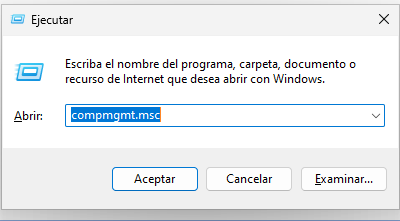
\includegraphics{png/WinRcompmgmt.png}

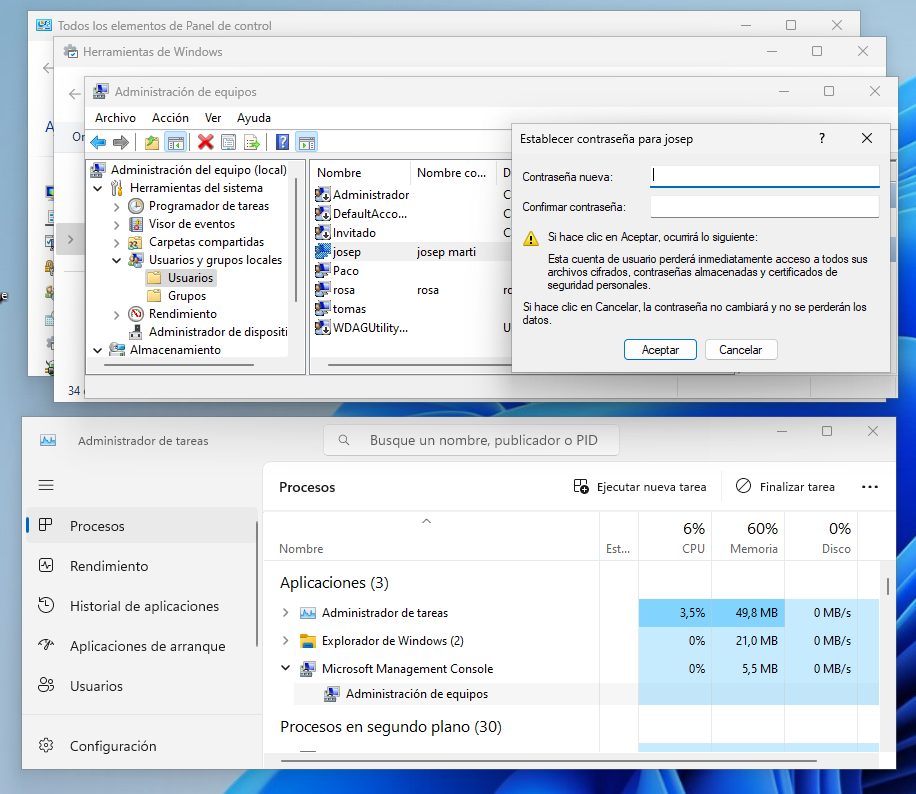
\includegraphics{png/2PaneldeControlHerramientasdeWindowsAdministradordeEquiposUsuariosygruposlocales.png}

\textbf{Avanç}

\begin{quote}
Les Microsoft Management Console (fitxers amb extensió \emph{.msc}) són
ferramentes gràfiques per a tasques d'administració i gestió dels
sistemes operatius Windows.

Podem trobar-les al directori d'instal·lació de Windows
\emph{c:\textbackslash windows\textbackslash system32}.
\end{quote}

Per accedir directament a la Consola d'Adminsitració d'Equips:

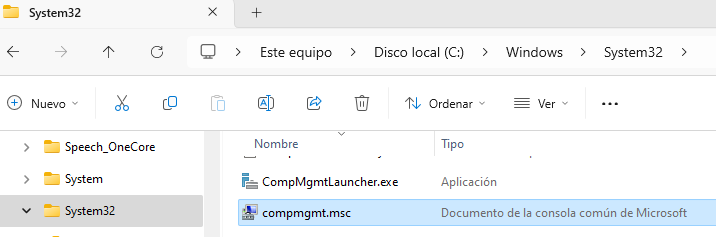
\includegraphics{png/fitxerCompmgmt.png}

\subsection{1.2 ALTRES OPCIONS}\label{altres-opcions}

Des del GUI podem fer algunes gestions amb els comptes d'usuaris amb
altres opcions gràfiques\ldots{}

\subsubsection{1.2.1 Panel de Control. Administrar
cuentas.}\label{panel-de-control.-administrar-cuentas.}

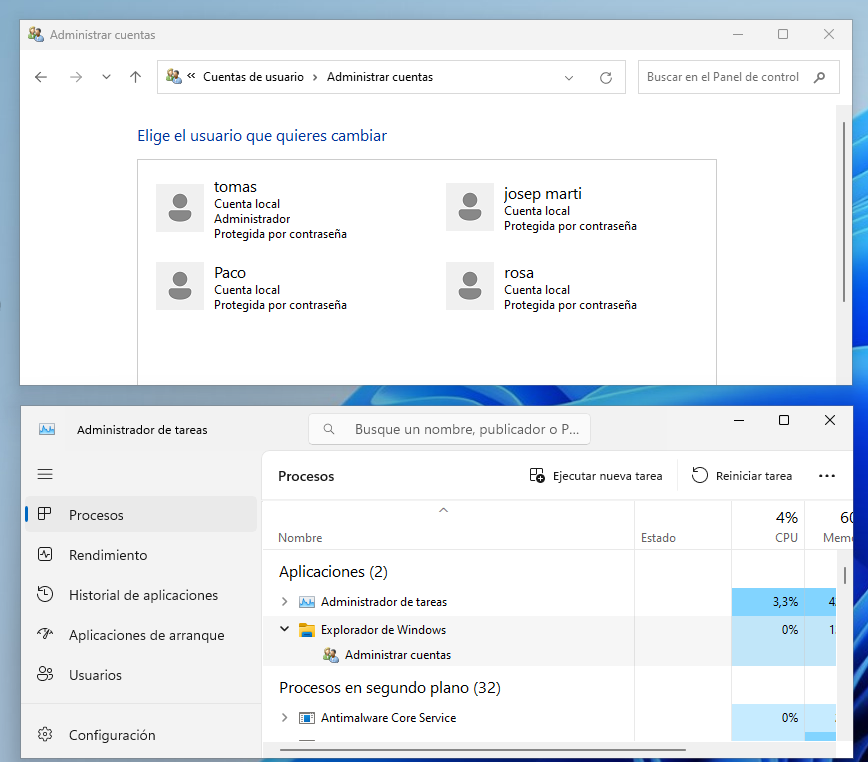
\includegraphics[width=0.8\textwidth,height=\textheight]{png/1PaneldeControlAdministrarCuentas.png}

En esta opció veien que podem canviar el tipus de compte
(Estàndar/Administrador) i poc més.
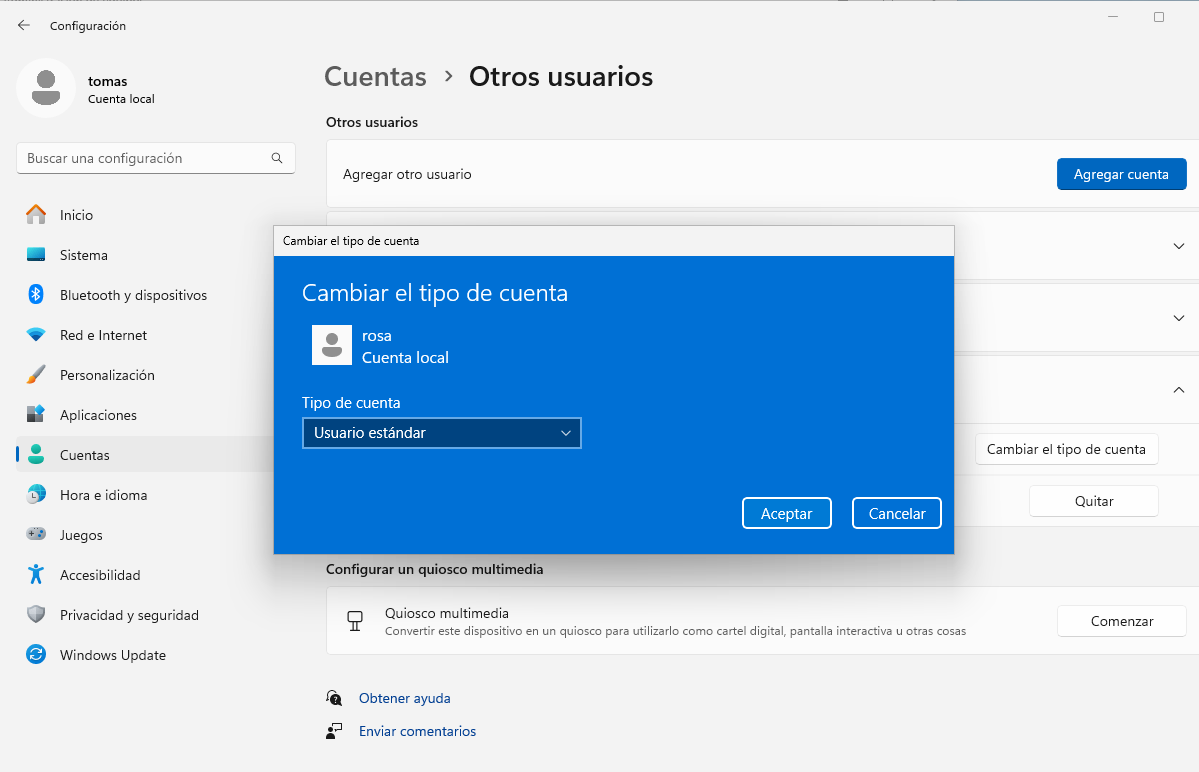
\includegraphics{png/cambiaTipoCuenta.png}

\textbf{Equivalències}

\begin{itemize}
\tightlist
\item
  El tipus per defecte ``Estándard'' equival al grup d'usuaris
  ``Usuarios''.
\item
  El tipus ``Administradores'' equival al grup d'usuaris
  ``Administradores''
\end{itemize}

\subsubsection{\texorpdfstring{1.2.2 Ferramenta
\emph{netplwiz.exe}}{1.2.2 Ferramenta netplwiz.exe}}\label{ferramenta-netplwiz.exe}

Windows + R i executem \textbf{netplwiz}.
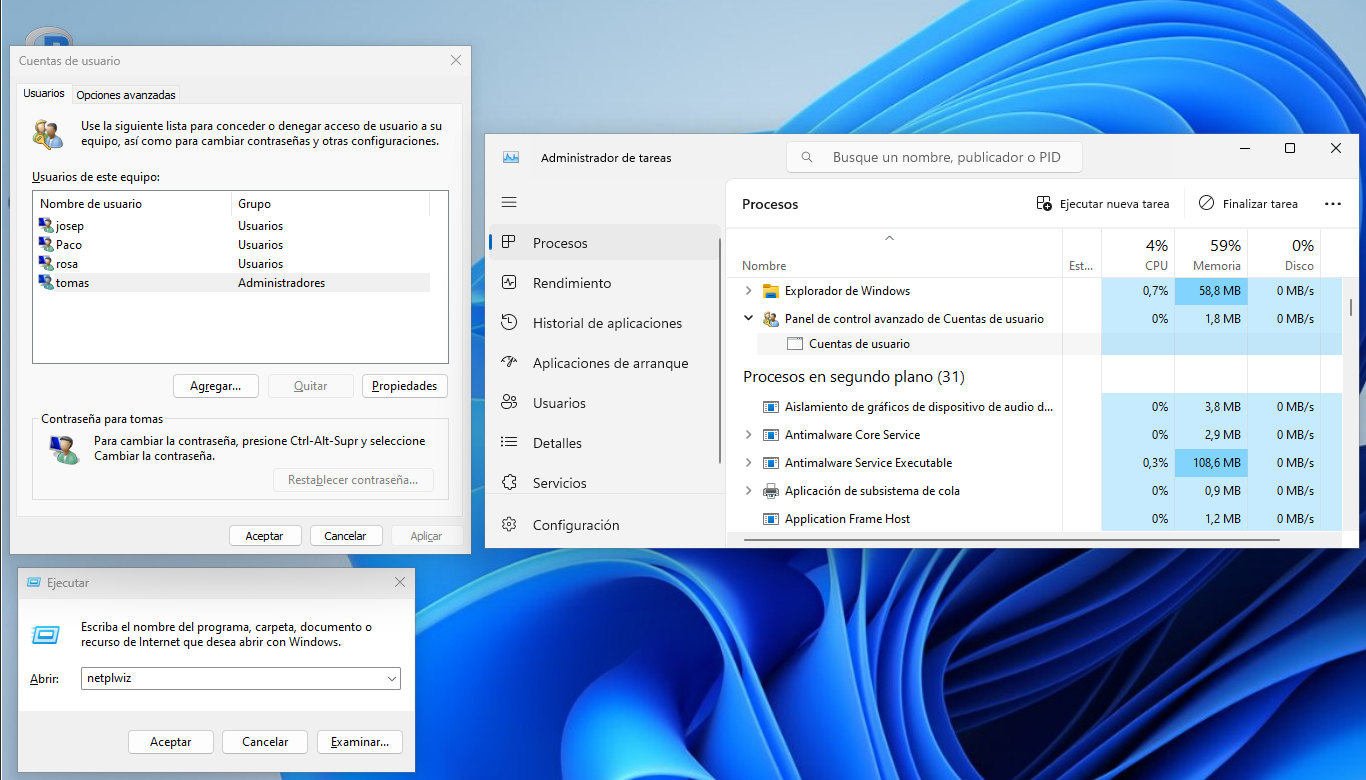
\includegraphics{png/3netplwiz.png}

En esta opció ens mostra els noms de grups d'usuaris als quals pertany
cada usuari. Ens permet afegir a algun grup distint d'Usuarios
(Estándar) i Administradores però no podem crear grups nous.

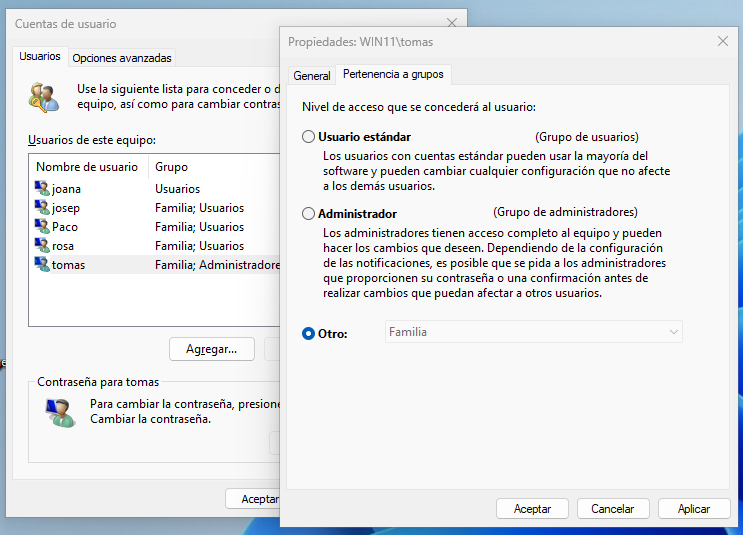
\includegraphics{png/propiedadesNetplwiz.png}

\textbf{Avanç}

\begin{quote}
Com podem observar a les imatges, cadascuna de les opcions gràfiques en
execució genera un procés distint.

A les imatges següents podem observar les tres alternatives gràfiques
obertes al mateix temps i fixar-nos-hi en les \textbf{tasques
\textgreater(procesos)} que s'hi veuen a l'\emph{Administrador de
Tasques}

També veiem com el component de Windows Consola de Equipos, en
executar-se dos vegades, genera dos processos.
\end{quote}

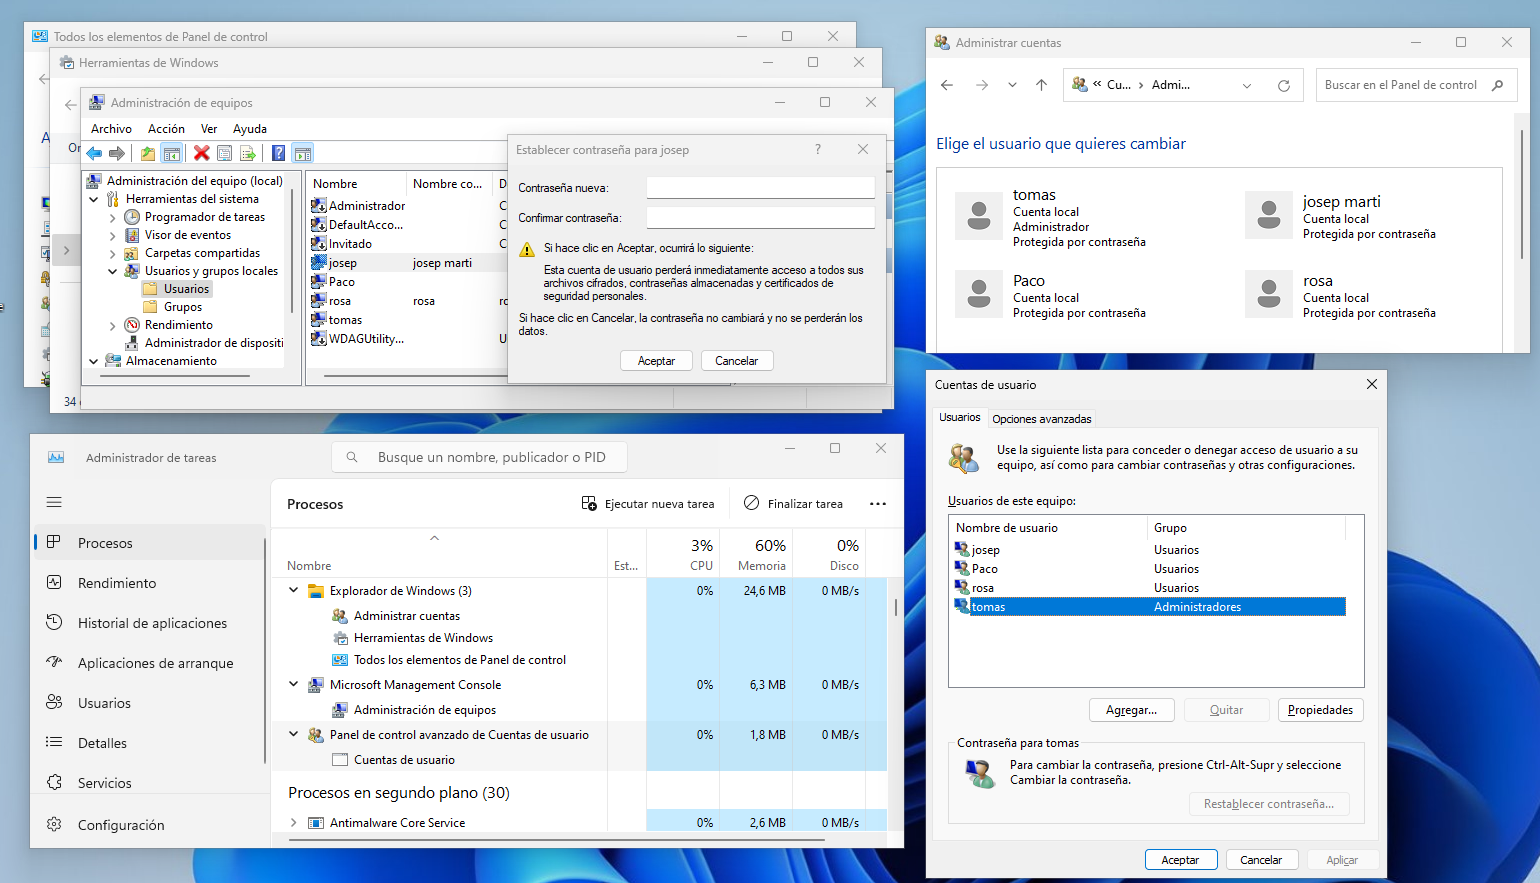
\includegraphics{png/123.png} !{[}{]})png/compmgmtTaskmanager.png)

\section{2 USUARIS I GRUPS}\label{usuaris-i-grups}

\subsection{2.1 Comptes per defecte}\label{comptes-per-defecte}

La instal·lació de Windows crea uns grups per defecte per al seu propi
funcionament.

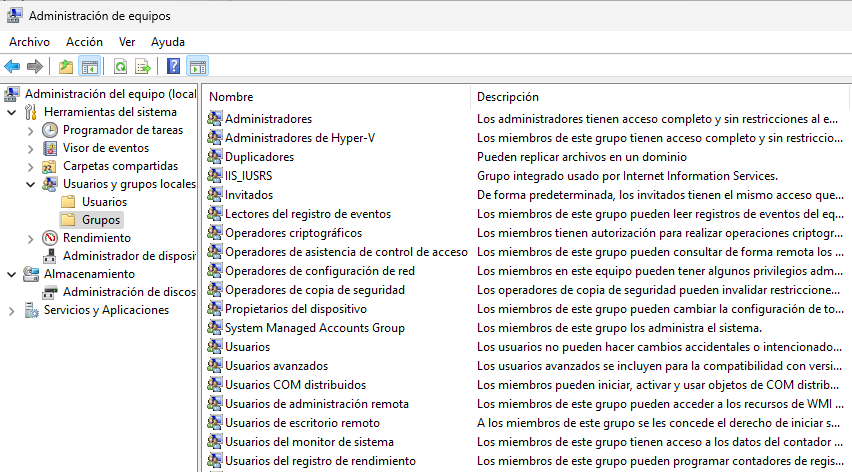
\includegraphics{png/grupsPerdefecte.png}

Ara ens centrarem en els dos principals que adés hem comentat:

\begin{itemize}
\item
  El Grup d'usuaris \textbf{Administradores}. Que tindran \textbf{drets}
  per realitzar qualsevol tasca que afecte a la configuració del sistema
  (SO, software, usuaris\ldots) i \textbf{permisos} per a modificar
  carpetes i fitxers (crear, eliminar, modificar contingut, canviar de
  propietari o permisos\ldots)
\item
  El Grup \textbf{Usuarios} A diferència dels anteriors, no tindran
  drets per fer certes modificació sobre la configuració (com dnar
  d'alta un usuaris o instal·lar). I només podran fer modificacions
  sobre fitxers i carpetes de la seua propietat.
\end{itemize}

Estos dos grups equivalen al ``tipo de cuenta'', \emph{Administrador} i
\emph{Estándar} comentatas al punt 1.2

També Windows crear en la instal·lació comptes d'usuari, per defecte
normalment inhabilitats, com \emph{Administrador, Invitado o
DefaulAccount}.

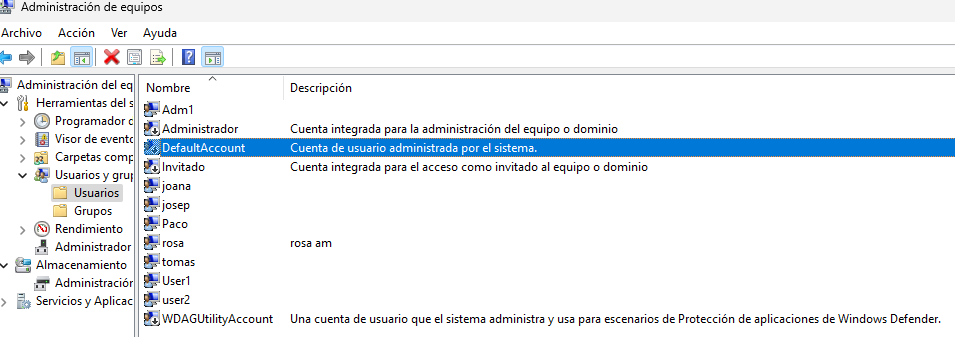
\includegraphics{png/usuarisCompmgmt.png}

\subsection{2.2 Nous comptes}\label{nous-comptes}

A nosaltres ens pot interessar crear altres grups d'usuaris amb
finalitats organitzatives; establir quines persones poden fer acciones
sobre el software (per exemple, instala·lacions), la configuració (per
exemple, crear un usuari) o poden fer modificacions en carpetes i
fitxers.

El que hem de tenir en compte és que, si bé per defecte un usuari és
\emph{administrador} o \emph{estándard} de forma exclusiva, podem crear
nous grups i incloure-hi els usuaris que vullguem. Fixem-nos a la imatge
següent. Observem que hem creat un grup ``Familia'' al qual hem afegit
un usuari que pertany al grup ``Administradores'' ( Tomas) i també un
usuari estandard del grup ``Usuarios''
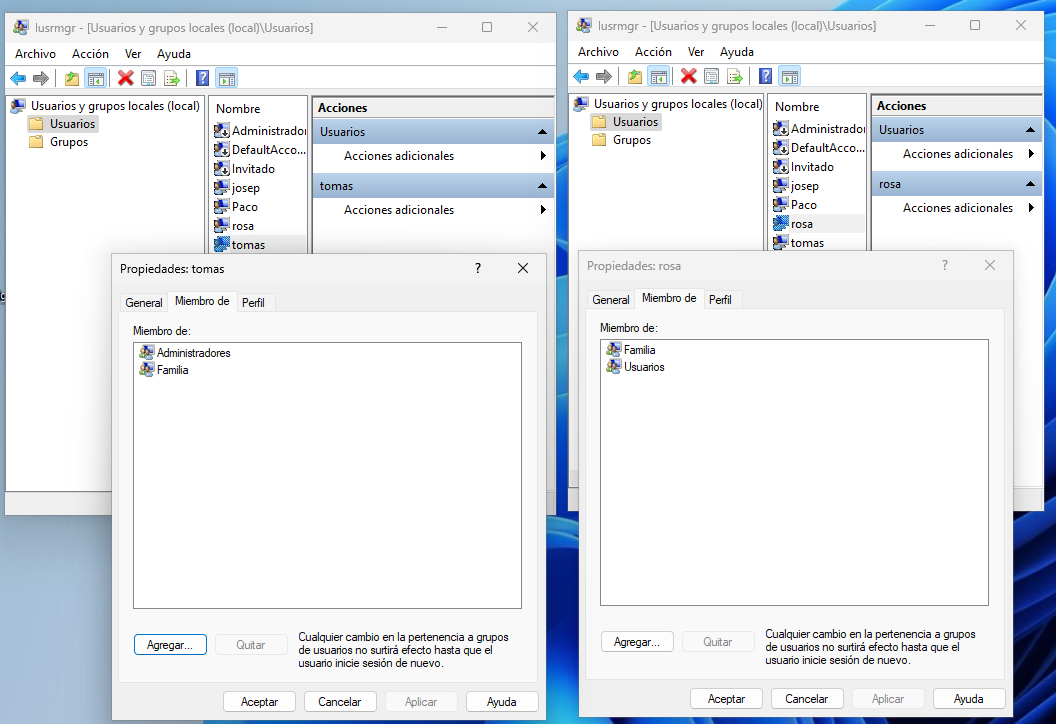
\includegraphics{png/mesdungrup.png}

\textbf{Avanç}

\begin{quote}
Un \textbf{permís} és una autorització que se li dóna a un usuari (o
grup) sobre carpetes o fitxer per a poder: 1. Llegir o 2. Escriure o 3.
Canviar els permisos (1 i 2) o el \emph{propietari} \textgreater{} unes
carpetes o fitxers

El \textbf{propietari} és, per defecte, l'usuari que ha creat la carpeta
o fitxer.
\end{quote}

\subsection{2.3 Acumulació de permisos de lectura, escriptura o
canvi}\label{acumulaciuxf3-de-permisos-de-lectura-escriptura-o-canvi}

Per tant, un mateix usuari pot pertànyer a més d'un grup. En estos
casos, els permisos de cadascun dels grups als quals pertany se sumen.
Ho estudiarem més avant.

\section{3. VISIÓ DES DE L'INTERFACE DE
COMANDAMENTS}\label{visiuxf3-des-de-linterface-de-comandaments}

Encara que en Windows11 serà més habitual treballar en l'entorn gràfic
hem de tenir sempre present que disposem de dos shells o interface de
comandaments:

\begin{itemize}
\tightlist
\item
  La consola de comandaments o cmd
\item
  Powershell
\end{itemize}

En una unitat següent s'estudiarà com crear modificar comptes des
d'estos entorns CLI. Ara, fem este avanç només per comprovar que els
usuaris estan creats però el seu perfil ( carpetes encara no ).

\subsection{3.1 Des de la consola CMD:}\label{des-de-la-consola-cmd}

Pulsem \emph{Win-R : cmd} i comprovem amb

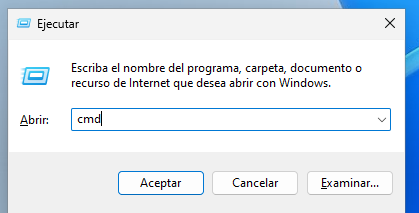
\includegraphics{png/WinRcmd.png}

\begin{Shaded}
\begin{Highlighting}[]
\NormalTok{net user}
\end{Highlighting}
\end{Shaded}

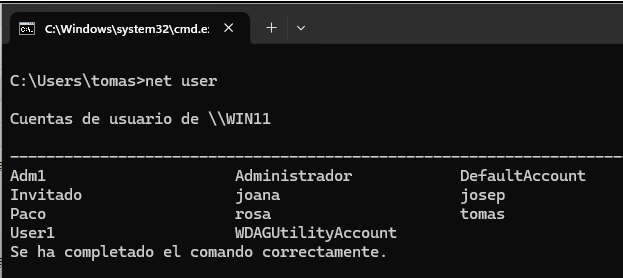
\includegraphics{png/netUser.png}

\begin{Shaded}
\begin{Highlighting}[]
\NormalTok{net localgroup}
\end{Highlighting}
\end{Shaded}

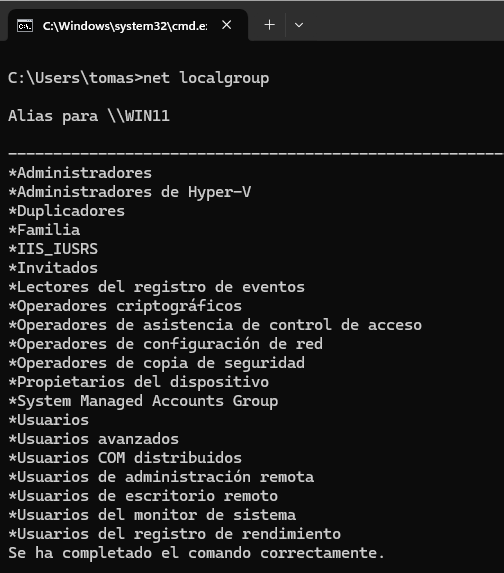
\includegraphics{png/netLocalGroup.png}

\subsection{3.2 Des de Powershell}\label{des-de-powershell}

Amb \emph{Win-R: powershell} o buscant

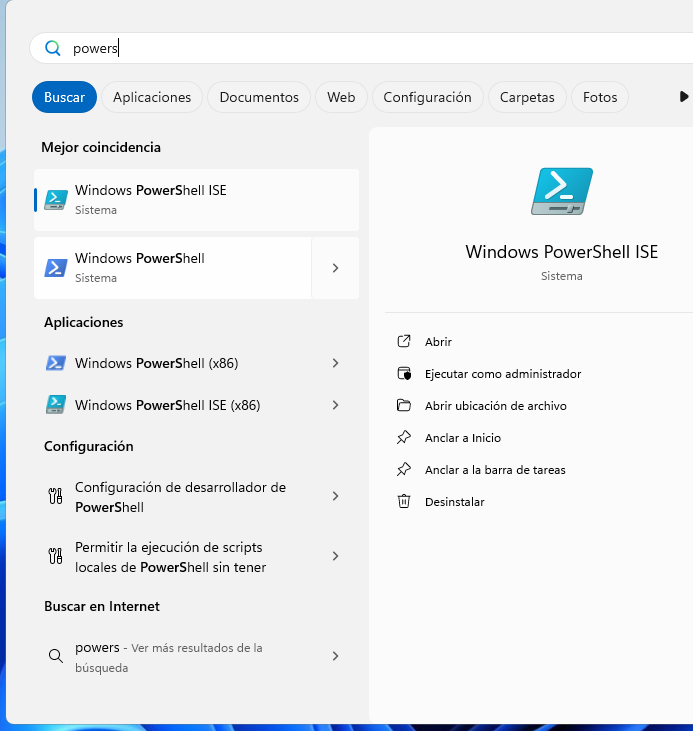
\includegraphics{png/powershell.png}

i comprovem amb

\begin{Shaded}
\begin{Highlighting}[]
\NormalTok{get{-}LocalUser}
\end{Highlighting}
\end{Shaded}

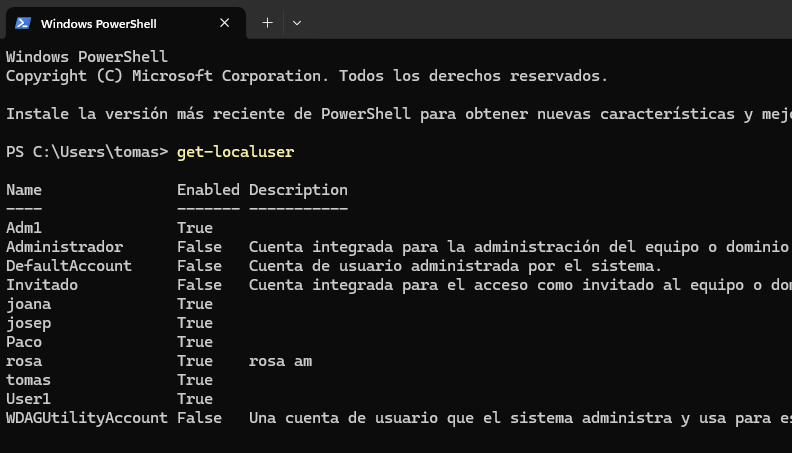
\includegraphics{png/get-LocalUser.png}

\begin{Shaded}
\begin{Highlighting}[]
\NormalTok{get{-}LocalGroup}
\end{Highlighting}
\end{Shaded}

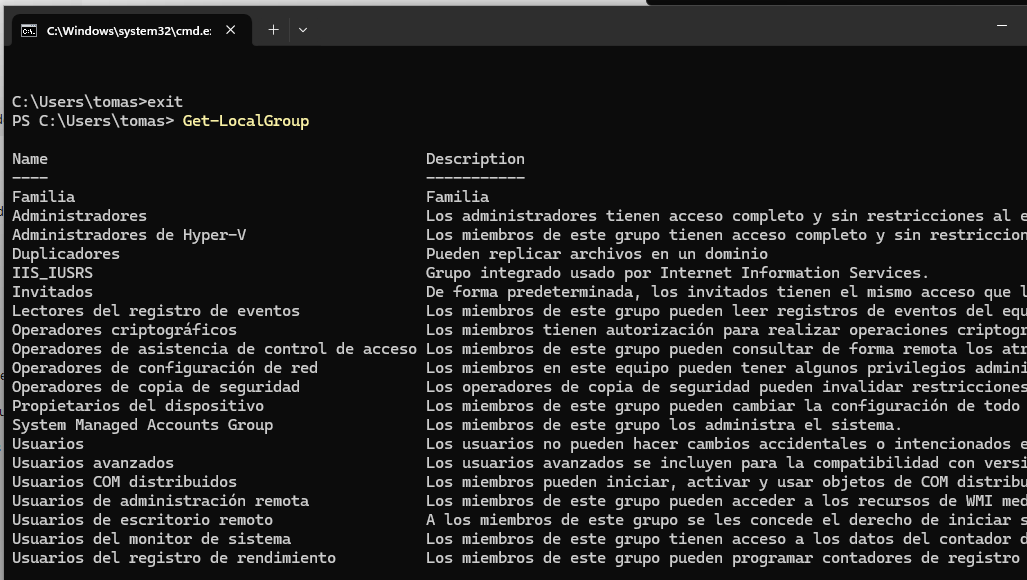
\includegraphics{png/get-LocalGroup.png}

\textbf{Avanç}

\begin{quote}
El Powershell és un potent shell de comandaments en línia amb un
lleguatge per a desenvolupar scripts (.ps1). Teniu un repositori per
aprendre'n més en este Git
\end{quote}

\section{5 VISIÓ AL REGISTRE del
SISTEMA}\label{visiuxf3-al-registre-del-sistema}

Observem com es registra al Registre del sistema els perfils (profiles)
de cada usuari.

\textbf{Avanç}

\begin{quote}
El Registre del sistema
(\emph{C:\textbackslash WINDOWS\textbackslash regedit.exe}) és un
component essencial de tots el sistemes Windows. Formalment és una base
de \textgreater dades jeràrquica que emmagatzema configuracions i
opcions del sistema operatiu i les aplicacions.
\end{quote}

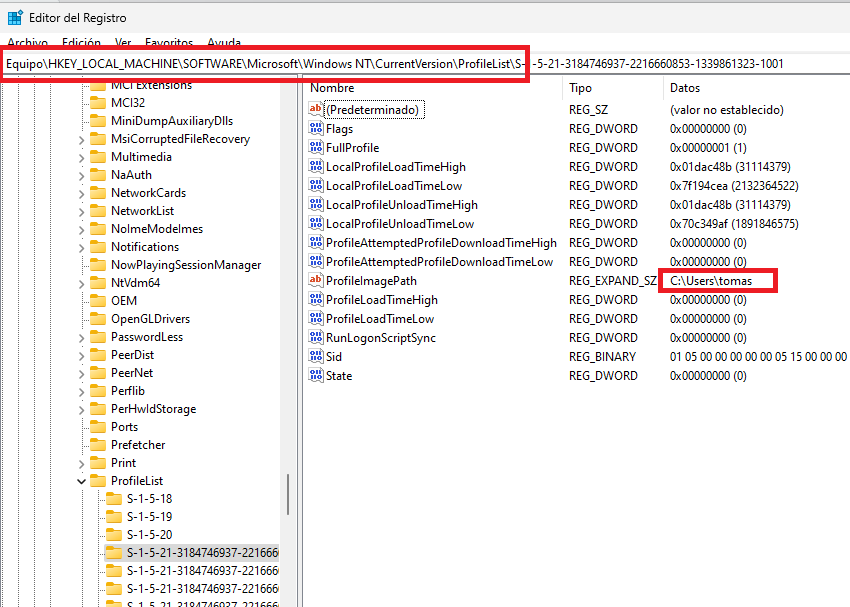
\includegraphics{png/regedit.png}

\section{4 PERFIL DE L'USUARI}\label{perfil-de-lusuari}

El perfil comprén tots els directoris ( ``Els meus Documents,
Descàrregues\ldots{}'') i altres característiques que són exlusives de
cada usuari o comuns.

Veiem les carpetes:

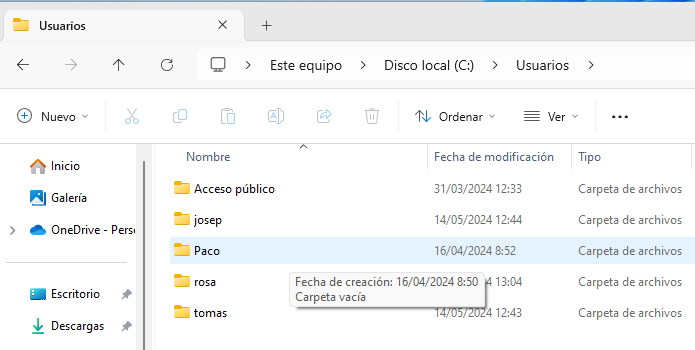
\includegraphics{png/users.png}

\subsection{4.1 Creació del perfil}\label{creaciuxf3-del-perfil}

Segurament si hem creat un usuari nou, haurem comprovat en l'anterior
punt que l'usuari acabat de crear:

\begin{itemize}
\tightlist
\item
  Apareix al GUI. Consola gràfica 8 compmgmt.msc ) i les altres opcions.
\item
  Apareix al CLI. \emph{net user} i \emph{get-localuser}
\item
  No apareix al registre del sistema la entrada a \emph{ProfileList}
\item
  No apareixen les carpetes de perfil personal a
  \emph{C:\textbackslash usuarios}
\end{itemize}

\textbf{NOTA}

\begin{quote}
Quan es crea el perfil de l'usuari? El perfil dels usuaris (
c:\textbackslash users\textbar usuari\textbackslash\ldots es crea quan,
una vegad creat, iniciem per primera vegada sessió amb ell. Notarem que
el primer inici de sessió es fa molt lent, sobretot si no hem desactivat
Cortana Com a nota podem avançar que en Linux veurem que ocorre el
mateix.
\end{quote}

Una vegada creat el perfil, podem entrar dins de la carpeta del nostre
usuari i observar tres subcarpetes:

\begin{itemize}
\tightlist
\item
  Default
\item
  Acceso Público
\item
  Una carpeta específica per cada usuari
\end{itemize}

Cadascuna té una funció que veiem tot seguit.

\subsection{4.1 Default}\label{default}

La carpeta \textbf{c:\textbackslash users\textbackslash Default}
{[}\^{}2{]} és una plantilla per a la creació de nous perfils d'usuari.
Conté configuracions i arxius predeterminats que es copien a qualsevol
nou compte d'usuari quan es crea. Ací es troben:

\begin{itemize}
\tightlist
\item
  \textbf{Configuracions del compte}: Preferències i configuracions
  d'aplicacions predeterminades.
\item
  \textbf{Carpetes d'usuari predeterminades}: Documents, Imatges,
  Música, Vídeos, Escriptori, Descàrregues, etc.
\item
  \textbf{Arxius de configuració}: Arxius de personalització de l'entorn
  d'usuari, com el fons d'escriptori, icones, accessos directes, etc.
\end{itemize}

Els nous usuaris de l'ordinador hereten estos arxius i configuracions la
primera vegada que inicien sessió.

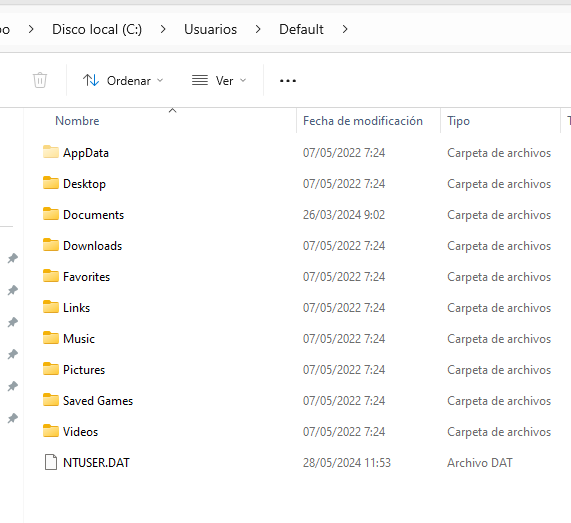
\includegraphics{png/CarpetesDefault.png}

\subsection{4.2 Acceso Público}\label{acceso-puxfablico}

La carpeta \textbf{Acceso Público} {[}\^{}3{]} Carpeta compartida
accessible per tots els usuaris de l'equip per compartir arxius sense
cap restricció.

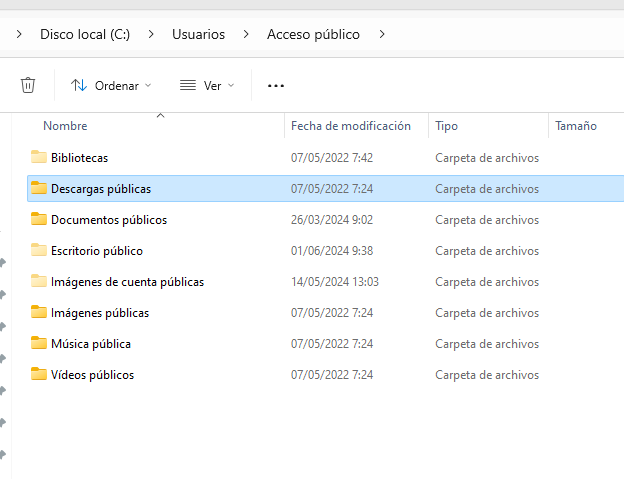
\includegraphics{png/CarpetesPublico.png}

\subsection{4.3 Carpeta de l'Usuari
Específic}\label{carpeta-de-lusuari-especuxedfic}

Cada usuari té la seva pròpia carpeta, que emmagatzema els seus arxius
personals i configuracions específiques. Esta carpeta inclou:

\begin{itemize}
\tightlist
\item
  \textbf{Carpetes personals}: Documents, Imatges, Música, Vídeos,
  Escriptori, Descàrregues.
\item
  \textbf{Configuracions d'usuari}: Configuracions específiques de
  l'usuari que afectaran a com pot usar el SO i aplicacions software.
\item
  \textbf{Arxius i configuracions personals}: Qualsevol arxiu que
  l'usuari guarde a seues carpetes personals i també les configuracions
  personalitzades.
\end{itemize}

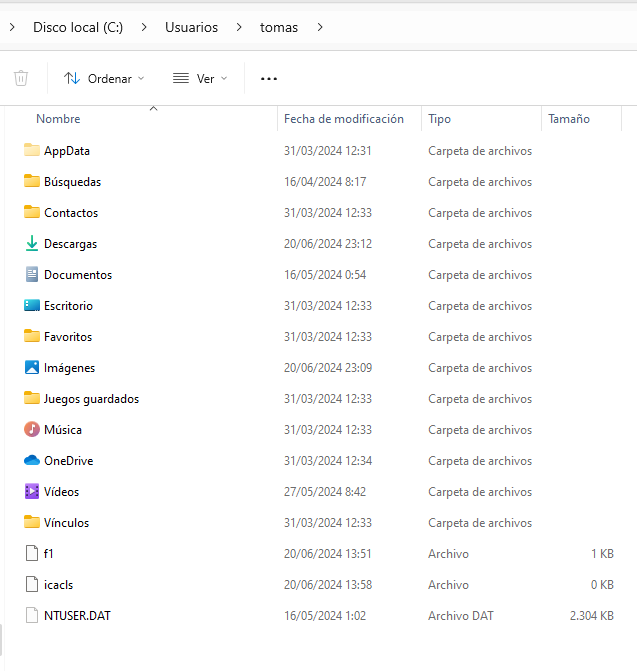
\includegraphics{png/CarpetesPerfil.png}

\begin{quote}
Només podrem entrar a carpeta d'altres usuaris si som Administrador. Es
proposa més avant una activitat per comprovar-ho.
\end{quote}

\newpage

\section{5 Activitats}\label{activitats}

\subsection{Activitat 1}\label{activitat-1}

\begin{enumerate}
\def\labelenumi{\arabic{enumi}.}
\tightlist
\item
  Des de la Consola gràfica, crea un usuari que pertanya al grup
  Administradores i un altre que no siga administrador i pertanyerà sols
  al grup d'usuaris:
\end{enumerate}

\begin{itemize}
\tightlist
\item
  Adm1
\item
  User1
\end{itemize}

\begin{enumerate}
\def\labelenumi{\arabic{enumi}.}
\setcounter{enumi}{1}
\item
  Assegura't que els dos usuaris hagen de canviar la contrassenya la
  primera vegada d'iniciar sessió en els dos usuaris.
\item
  Inicia sessió, amb l'usuari \emph{Adm1}.

  3.1 Observa els continguts de les carpetes
  C:\textbackslash Users\textbackslash Adm1 i anota, si existeixen, qué
  contenen.

  3.2 Observa els continguts de les carpetes
  C:\textbackslash Users\textbackslash User1 i anota, si existeixen, qué
  contenen

  3.3 Crea un fitxer \emph{Telefons.txt} a la carpeta personal de Adm1
  C:\textbackslash users\textbackslash Public\textbackslash Documents

  3.4 Crea una carpeta \emph{Diari} a la carpeta
  C:\textbackslash Users\textbackslash Default\textbackslash Desktop
\item
  Inicia sessió amb \emph{User1}. Ara comprovarem l'efecte dels canvis
  fets adés en este usuari nou.

  4.1 Comprova si apareix la carpeta \emph{Diari} a l'escriptori

  4.2 Està disponible
  C:\textbackslash users\textbackslash Public\textbackslash Documents\textbackslash Telefons.txt

  4.3 Entra al perfil de User1
  C:\textbackslash users\textbackslash User1 i observa el contingut de
  les carpetes
\item
  Sense tancar sessió (sessió de \emph{User1} ) intenta crear un grup
  d'usuaris amb el nom de \emph{Botiga}

  5.1 Afig dins d'ell els dos usuaris \emph{User1 i Adm1}

  5.2 Crea un tercer usuari estàndard \emph{User2} i afig-lo al grup
  \emph{Botiga}

  5.3 Descarrega't un foto d'una botiga que usaran tots els usuaris. En
  quina creus deuries alçar-la tractant-se d'una imatge per compartir?
\end{enumerate}

\end{document}
